\documentclass[12pt]{article}
\usepackage{graphicx}
\usepackage{algpseudocode}
\usepackage{algorithm}
\usepackage{booktabs}
\usepackage[style=alphabetic, backend=biber]{biblatex}

\graphicspath{ {./images/} }

\addbibresource{references.bib}

% Preamble
\setlength{\parindent}{0pt}
\linespread{1.5}

% Document Information
\title{Ray Tracing Voxels with Hardware Acceleration in Real-Time \\
    \vspace{1cm}
    \large Is hardware accelerated voxel ray possible on consumer hardware for real-time applications?}
\author{Srijan Dhungana}
\date{2024}

% Begin Document
\begin{document}

% Title Page
\maketitle
\clearpage

% Table of Contents
\tableofcontents
\clearpage


\clearpage

\section{Motivation}

My first introduction to ray tracing was when NVIDIA announced their RTX series GPUs in 2018.
The idea of simulating light rays in real-time was unreal and the results were stunning.
I wanted to make my own hardware ray tracer and so I was introduced to computer graphics.
The aesthetics of voxels based games have been fascinating and I wanted to combine the two.
However, when researching, I found that there was no performance analysis of hardware accelerated voxel ray tracing.

\section{Introduction}

\subsection{Ray Tracing}

Ray tracing is a method to calculate where a given ray (line), intersects
with the environment. This is useful to simulate light rays because of how light behaves. It is used in film
production, video games, optics, medical imaging, architectural visualization,
and many other fields. Physically light rays bounce in the environment, thus
ray tracing is used to calculate the position of intersection where a light ray
hits the environment. Then the programmer is free to repeat the process
and simulate the ray bouncing off into other directions. This process is a
highly parallelizable process, thus it is perfectly suited for GPUs which have
thousands of cores. However, due to how computationally expensive the
process is, it is not feasible to do in real-time without dedicated hardware
acceleration. Due to those limitations, it was only used in non-real-time
applications such as film production. Hardware acceleration ray tracing was introduced in 2018 by Nvidia.
Since then, ray tracing has been possible in real-time and further supported by AMD and
Intel GPUs. This has allowed real-time applications to leverage ray-tracing such as video games.

\subsection{Voxels}

Voxels are a way to represent 3D data. It is similar to pixels in 2D images,
but in 3D space. Essentially, voxels are cubes that are located in 3D space.
They are used in visualization applications, and video games; they have
similar applications to ray tracing. Voxels are convenient, because they represent
volumetric data, which is difficult to represent with traditional with polygons that the GPU is designed to handle.
Environment scans and medical imaging data are examples of volumetric data.
For example, LiDAR sensors are used to scan the environment and create volumetric data.
This data can be represented as voxels, and then used in simulations or visualizations.
Each voxel can contain data, such as color, or density captured from the sensors,
which can be utilized in simulations or visualizations.

\subsection{Research Question}

The research question is: Is hardware accelerated voxel ray possible on consumer hardware for real-time applications?
Real-time applications considered are video games, and visualizations that utilize volumetric data in the form of voxels.
These are the factors that will be considered when evaluating the possibility:
\begin{itemize}
    \itemsep0em
    \item Can it handle a reasonable number of voxels? (3-15 Million)
    \item Does it exceed the memory budget? (4GB)
\end{itemize}

Moreover, this essay attempts to analyze the GPU hardware bottlenecks that limit the performance of voxel ray tracing.

\section{Background Information}

\subsection{Mathematics of Ray Tracing}
\subsubsection{The Ray Equation}

A ray is defined by a point and a direction. The equation of a ray is given by:

\begin{equation}
    R(t) = \vec{o} + t\vec{d}
\end{equation}

where $\vec{o}$ is the origin of the ray, $\vec{d}$ is the direction of the ray, and $t$ is the distance from the origin.
The function $R(t)$ gives the position of the ray at distance $t$ from the origin.
With this equation, any point along the ray can calculated.

\subsubsection{The Intersection Function}

Whenever a ray intersects with a surface, the point of intersection is given by the equation:

\begin{equation}
    R(t) = I(t)
\end{equation}

where $I(t)$ is the intersection function of the surface. To locate the point of intersection,
solving for $t$ is necessary by equating the ray equation with the intersection function. 
If there are solutions for $t$, then the ray intersects with the surface. However, 
if $t$ is negative, then the intersection is opposite to the direction of the ray, which is not desired,
hence negative solutions are discarded. The closest hit is usually desired thus smallest non-negative $t$ is chosen.

\subsection{Ray Tracing Algorithm}

The ray tracing algorithm is a recursive algorithm that calculates the color of a pixel by tracing rays into the scene from a virtual camera.
Ray tracing algorithm is as follows:

\begin{algorithm}[H]
\caption{Ray Tracing Algorithm}
\label{alg:TraceRay}
\tiny
\begin{algorithmic}[0]

\State $Emissive \gets 0$
\Procedure{TraceRay}{$direction, depth$}

    \If{$depth = 0$}
        \State \Return $0$ \Comment {Hit no light source after maximum depth}
    \EndIf

    \State $closestHit \gets \infty$
    \State $hitObject \gets null$

    \For{$object$ in $scene$}
        \State $hit \gets object.Intersect(direction)$
        \If{$hit < closestHit$}
            \State $closestHit \gets hit$
            \State $hitObject \gets object$
        \EndIf
    \EndFor

    \If{$closestHit = \infty$}
        \State $Emissive \gets 1$ \Comment {Sky is a light source}
        \State \Return $background$
    \EndIf
    \State $Emissive \gets hitObject.emissive$
    \If {$hitObject.emissive$} \Comment {If the object is a light source}
        \State \Return $hitObject.Color$
    \EndIf

    \State $newDirection \gets randomDirectionFromObject(hitObject)$

    \State \Return $object.Color * TraceRay(newDirection, depth - 1)$

\EndProcedure

\For{$pixel$ in $image$}
    \State $direction \gets getDirectionForPixel(pixel)$
    \State $color \gets TraceRay(direction, maxDepth) * Emissive$
    \State $image[pixel] \gets color$
    \State $Emissive \gets 0$ \Comment{Reset Emissive}
\EndFor

\end{algorithmic}
\end{algorithm}

The pseudocode in Algorithm \ref{alg:TraceRay} shows a simple recursive algorithm for ray tracing.
It finds the closest hit in the scene and if the object is emissive (light source), then the pixel is illuminated.
Note that if the path doesn't hit a light source, the path color is multiplied by 0, which results in a black pixel.

This recursive algorithm is repeated thousands of times for each pixel and the result is an image.
Even then, the image is an approximation of the real world because the algorithm only simulates a fraction of all the possible paths.
In this essay, this is the algorithm that will be used to simulate the paths of the rays.
This algorithm is split into multiple stages in the GPU.

\begin{figure}[H]
    \begin{center}
        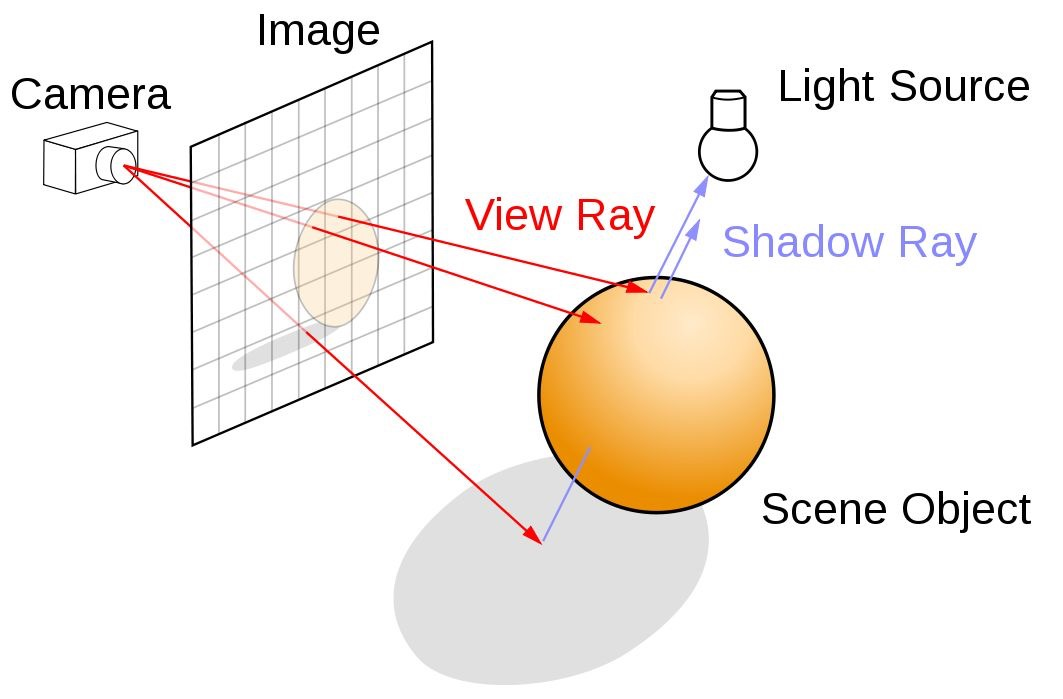
\includegraphics[scale=0.22]{RayTracingImage}
    \end{center}
    \caption{Simplified visualization of the Algorithm \ref{alg:TraceRay}. \parencite{NVIDIA:Raytracing}}
    \label{fig:RayTracingImage}
\end{figure}

\subsection{Process of Ray Tracing on Hardware}
In this section, the ray tracing process on hardware is explained.

\subsubsection{Acceleration Structures}
Without any optimization algorithms, the intersection function has to be solved for every primitive in the scene to determine the closest hit. 
Primitives are smallest building blocks of the scene. The GPU only accepts triangles and axis aligned bounding boxes (AABB) as primitives.
AABBs are cuboids that are aligned in the x, y, and z axes.
Solving the intersection function for every primitive is computationally expensive for scenes with millions of primitives.
Hence, acceleration structures (AS) are used to reduce the number of times the intersection function is solved.
These structures are usually bounding volume hierarchies (BVH) that subdivide the scene into smaller parts until the smallest primitives are reached \parencite{NVIDIA:Raytracing}.
Bounding volumes are AABBs that enclose the primitives.
This method logarithmically decreases the number computation required to find the closest hit.

\begin{figure}[H]
    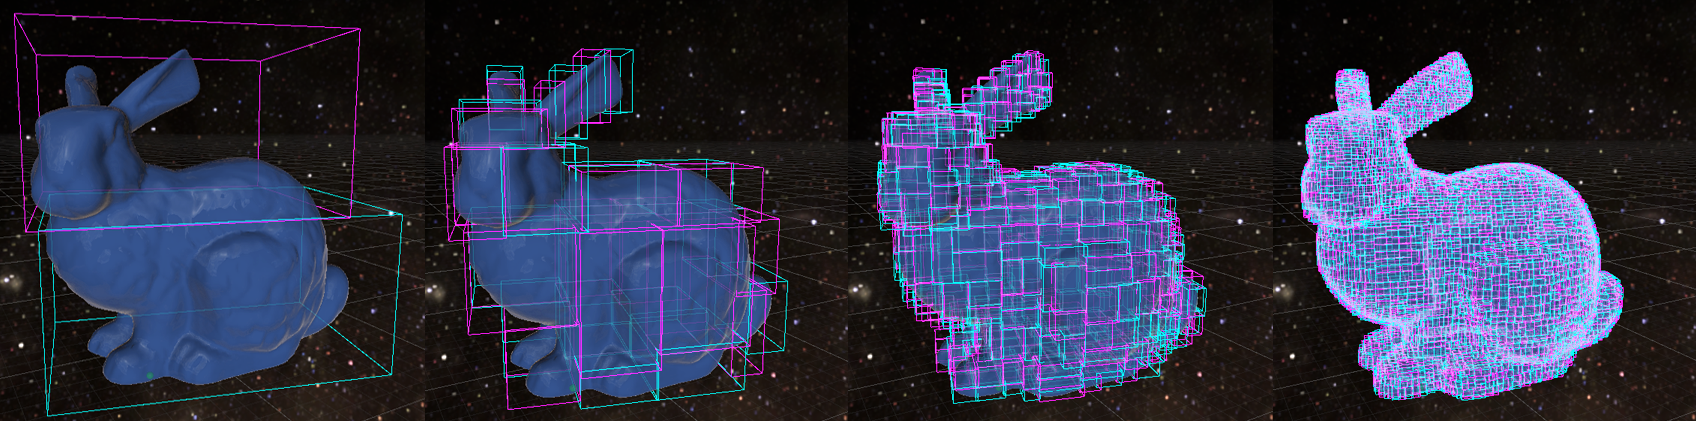
\includegraphics[scale=0.22]{BVH-Visualization}
    \caption{
        Bounding Volume Hierarchy of a bunny. 
        The bunny is divided into smaller bounding volumes until the individual triangles are reached.
        \parencite{Medium:BVH-Visualization}
        }
    \label{fig:BVH-Visualization}
\end{figure}

The BVH is a non-trivial tree structure that is constructed every object in the scene and requires ample memory.
When a ray enters a bounding volume (box), it is guaranteed that only the primitives inside the bounding volume are potential hits.
If the ray does not hit any primitives inside the bounding volume, then the ray goes to the previous bounding volume in the hierarchy and continues
to search for hits. This is repeated until the ray hits a primitive or exits the scene.

\subsubsection{Ray Tracing Pipeline}

The ray tracing pipeline is a series of steps that the GPU follows to use ray tracing.

\begin{figure}[H]
    \begin{center}
        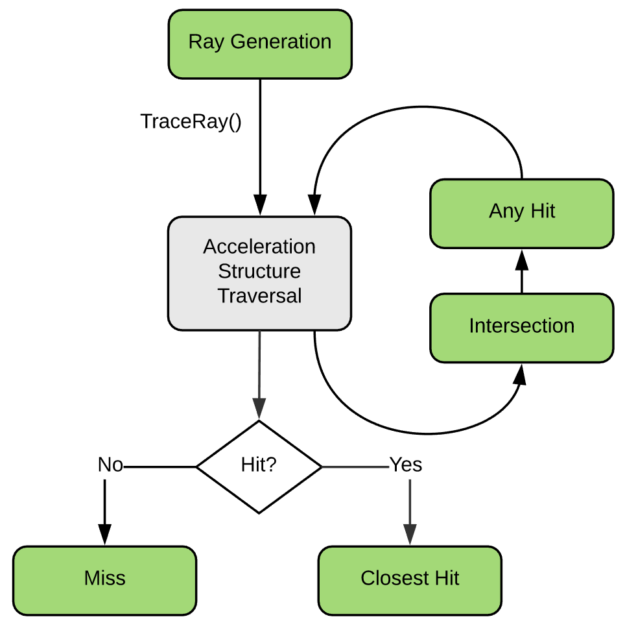
\includegraphics[scale=0.25]{RayTracing-Pipeline}
    \end{center}
    \caption{
        The Ray Tracing Pipeline.
        Green boxes are programmable functions and grey boxes are fixed functions in hardware.
        \parencite{NVIDIA:DXR-Intro}
        }
    \label{fig:RayTracing-Pipeline}
\end{figure}

The ray tracing pipeline is shown in Figure \ref{fig:RayTracing-Pipeline}. 
Nearly all the steps in the pipeline are programmable, which allows the user to customize the pipeline.
Ray generation is the first step where the rays are generated from the camera in the correct direction and location.
The hardware acceleration structure traversal is the most critical step because it requires the most computation.
It is fully implemented in hardware and is not programmable until it reaches the leaf nodes of the BVH, after which the intersection stage is programmable.
For triangles primitives, the intersection stage is fixed in hardware, meaning it is not programmable.
For AABB primitives, the stage is programmable, which allows the user to run their own intersection function.
This is because, AABBs are meant to enclose user defined primitives.
For example, a sphere can be enclosed in an AABB and the acceleration structure traversal is hardware accelerated
until the AABB is hit. After hitting the AABB, the user defined intersection function for the sphere is invoked,
allowing the user to run their own sphere intersection function \parencite{NVIDIA:BVH-Patent}.
The intersection function needs to report the $t$ value of $R(t) = I(t)$ if there is an intersection.
The acceleration structure traversal and intersection stage are repeated until the closest hit is found,
that is the smallest non-negative $t$ value. Then the closest hit stage is invoked with the information
about the hit location and the object that was hit.
Closest hit can be used to shade the hit point and even generate new rays into different directions to simulate light bouncing. 

The anyhit stage is used to accept or discard hits. However, the anyhit stage is optional and can be omitted.
If no hit is found, the miss stage is invoked.
 Miss stage is used to shade the background if no hit is found.
\parencite{NVIDIA:RTGems2}

\section{Methodology}

\subsection{Utilizing Hardware Acceleration}

This essay will use AABBs as voxels, because the GPU only accepts either triangles or AABBs as primitives.
Voxels are easily represented as AABBs, because both are cuboids. 
The other alternative, representing voxels as triangles is not practical. Voxels have 6 faces, 2 triangles
are needed to represent each face, thus 12 triangles are needed to represent a voxel. This amounts to 
inefficent memory usage and computation. Usage of AABBs implies that the user has to program the intersection stage.

Acceleration structure generation is a black box in graphics APIs, where 
the primitives are supplied to the GPU and it constructs the AS. This is convenient to both the programmers and vendors, because
vendors can optimize the AS construction and traversal for their hardware and users are ensured that the AS has optimal performance.

\subsection{Optimizing the Intersection Function}
\label{sec:OptimizingIntersection}

There are complications to representing voxels as AABBs, because AABBs were meant to be extremely flexible to 
enclose any user defined primitive. This section provides an optimization for the intersection stage,
which involves approximating the closest hit.

\begin{figure}[H]
    \begin{center}
        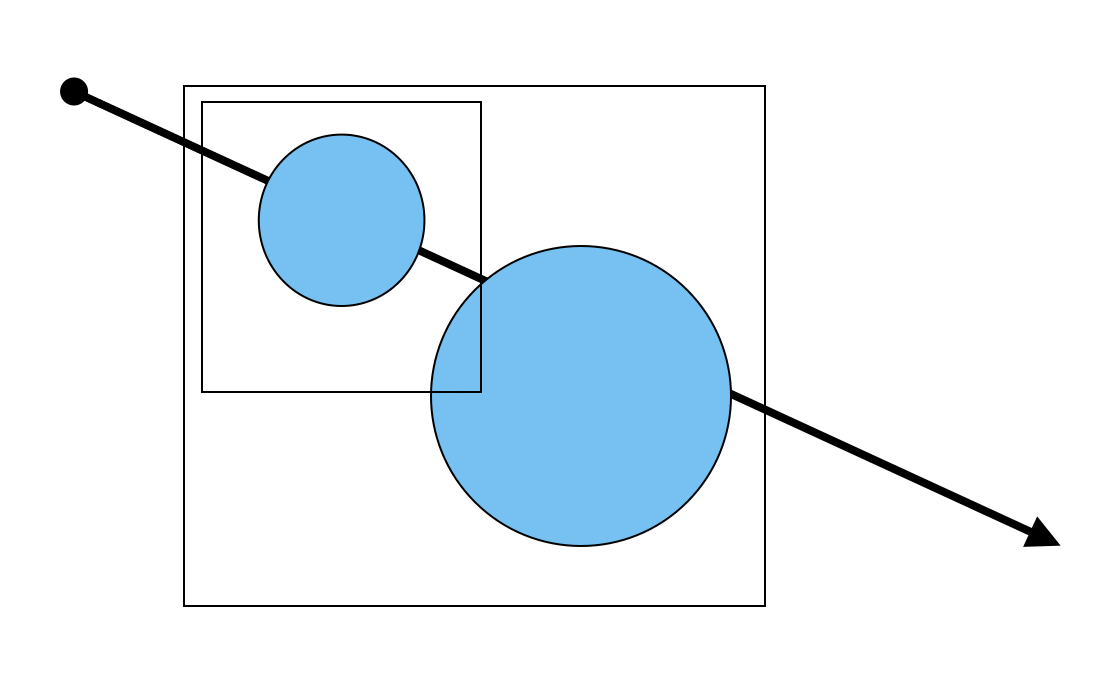
\includegraphics[scale=0.5]{ClosestHit-Ambigous}
    \end{center}
    \caption{
        A scenario where the closest hit is not known by the GPU without invoking the user's intersection function.
        Even though the larger AABB is closer to the ray origin, the smaller AABB has a closer intersection
        with it's enclosed object.
    }
    \label{fig:ClosestHit-Ambigous}
\end{figure}

Figure \ref{fig:ClosestHit-Ambigous} shows a scenario where the GPU itself cannot determine the closest candidate just by
taking into account the AABBs. Because of this, every AABB along the ray has to be tested for intersection, which 
means the intersection stage can be invoked multiple times. For maximum performance, the the GPU should minimize 
the number of calculations performed in the intersection stage.

\begin{figure}[H]
    \begin{center}
        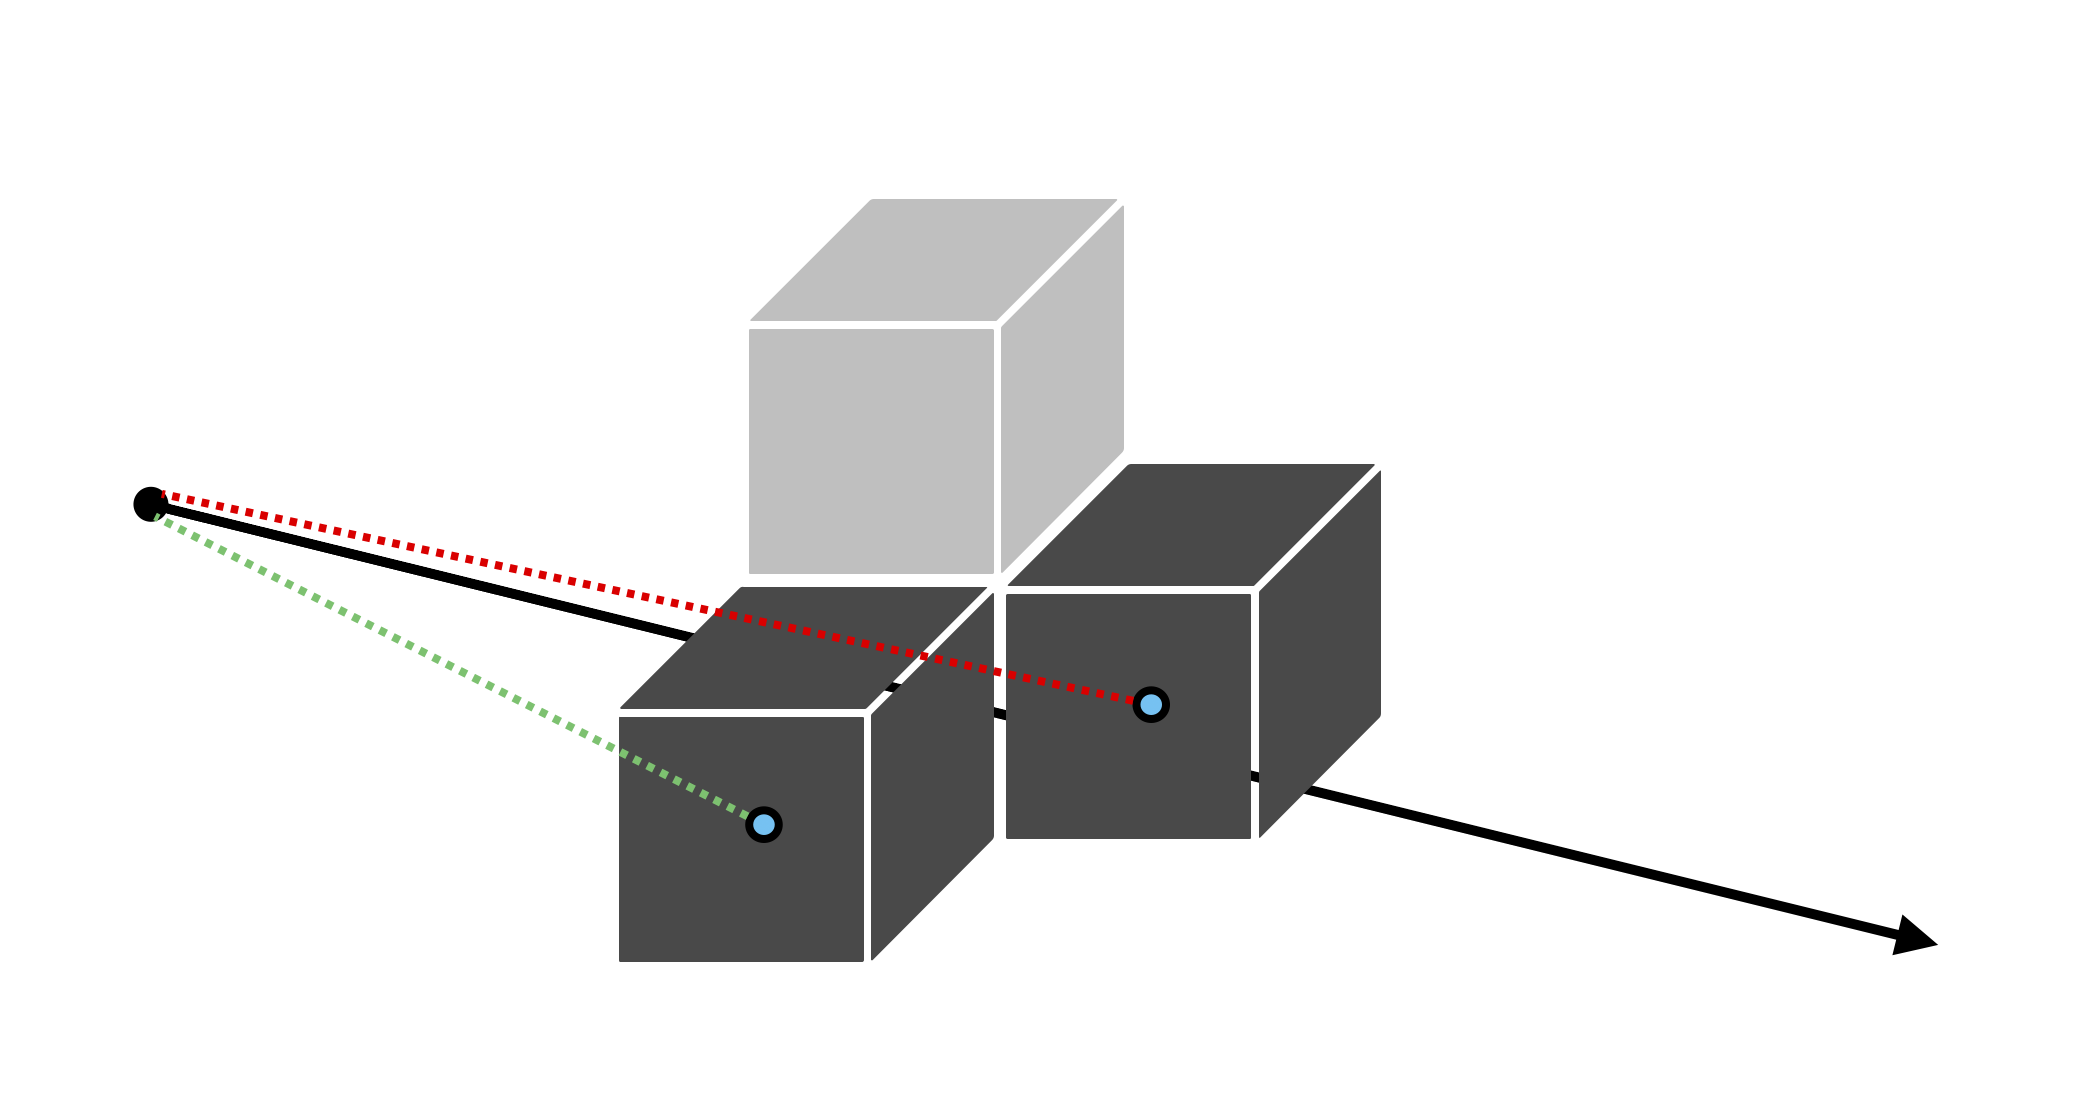
\includegraphics[scale=0.22]{ClosestHit-Approx}
    \end{center}
    \caption{
        Solving for closest hit candidate without an intersection test.
        Instead the distance from the ray origin to the AABB is calculated and the closest candidate is selected.
        }
    \label{fig:ClosestHit-Approx}
\end{figure}

Making the intersection stage efficient is trivial in this case.
Finding an exact solution for every candidate is not necessary. 
The GPU will pick the candidate with the smallest $t$ value reported, which can be approximated.
After the closest candidate is picked, the exact intersection point can be solved in the closest hit stage.
Only one exact solution is calculated, which is much more efficient than solving for every candidate.
Figure \ref{fig:ClosestHit-Approx} shows solving for the closest candiate without an intersection test.
In this case, since the voxels are never overlapping each other and of uniform size, the scenario in Figure \ref{fig:ClosestHit-Ambigous} is not possible.
Using this assumption, the closest voxel along the ray is guaranteed to have the closest intersection.
This method only involves calculating the distance from the ray origin to the voxel center and selecting the closest candidate.
Fetching the voxel center is an array fetch and calculating the distance is a simple vector instruction, which is very fast.
The candidate with the smallest distance is selected as the closest hit, as described in the previous section.
In the closest hit stage, there is enough information to calculate the exact intersection point.

\subsection{Memory Consumption}

The memory consumption is greater for AABBs than for voxels.
Unfortunately, the GPU requires AABBs to be used for hardware acceleration.
AABBs need two 3D vectors to represent the minimum and maximum points of the cuboid.
This is 6 floats or 24 bytes per AABB.
If there is a scene with 1 million voxels, then the memory consumption would be 24MB.
This may not sound like much, however the AS has extra AABBs for the hierarchy, which will add upto more memory.
To do lighting calculations and other operations, the user would need to access the data inside the voxels.
The graphics API does not allow accessing the data inside the AS, so there would be duplicated data.

\subsection{Data Collection}
Data collection to analyze the performance is done by measuring the frame time and frames per second (FPS)
The following configuration is run on 3 different scenes with varying number of voxels.
These scenes are real world scans that were in the form of polygons.
They were converted to voxels by using FileToVox software \parencite{Github:FileToVox}.

\begin{itemize}
    \itemsep0em
    \item New York City: 4.3 million voxels \parencite{SketchFab:NewYorkCity}
    \item Operating Room: 5.2 million voxels \parencite{SketchFab:OperatingRoom}
    \item Church: 13.6 million voxels \parencite{SketchFab:Church}
\end{itemize}

The ray tracing algorithm is run for 4096 frames, and the average frame time is calculated.
Each ray can at most bounce 4 times, so the recursion depth is 4.
From the average frame time, the average frames per second is calculated, by $FPS = \frac{1}{Average Frame Time}$.

Two methods of intersection tests are used:
\begin{itemize}
    \itemsep0em
    \item Exact Intersection: The exact intersection is calculated for every voxel.
    \item Approximate Intersection: The closest hit is approximated and the exact intersection is calculated in the closest hit stage.
    Described in Section \ref{sec:OptimizingIntersection}.
\end{itemize}

\section{Results}

This essay's analysis is based upon NVIDIA 3060ti GPU on Windows 11 using DirectX 12.
Results may vary on different hardware and software configurations.

\subsection{Driver Conformance}

Graphics APIs are high level interfaces that allow the user to interact with the GPU,
and the driver acts as a middleman between the API and the GPU Hardware.
The code used in this essay has been written on Vulkan, and DirectX 12 graphics APIs,
and the NVIDIA's GPU driver has been found not to conform strictly to either of the specifications.

Wrong information about the AABB that was hit is passed to the intersection and closest hit stages.
The driver is merging voxels that are close to each other, into a single wide AABB.
The user does not know that the AABB was merged and expects it to act as individual voxels.
It is important to note, that the driver may merge the AABBs for optimization, but it should still act as if the AABBs were not merged.

\begin{figure}[H]
    \begin{center}
        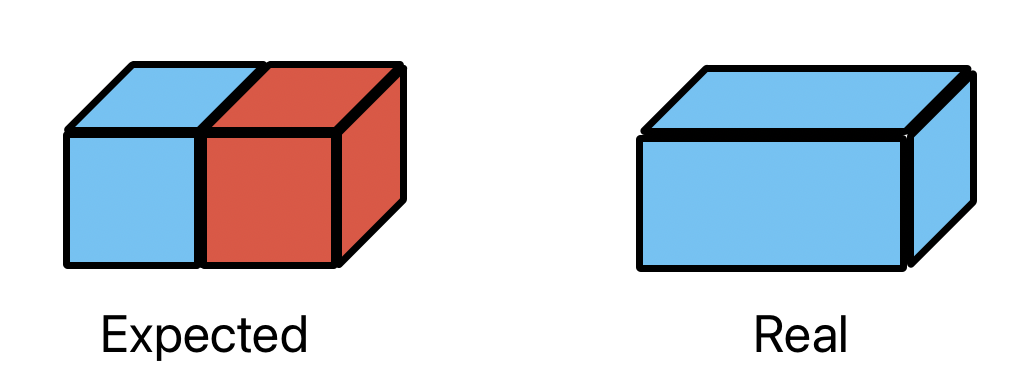
\includegraphics[scale=0.5]{Voxel-Merging}
    \end{center}
    \caption{
        The expected behavior compared to the real behavior.
        }
        \label{fig:Voxel-Merging}
\end{figure}
    
The merged AABB in Figure \ref{fig:Voxel-Merging} is blue,
because the driver reports that the primitive hit is the blue voxel even for the right side of the merged AABB.

The exact intersection method does not suffer from this issue, however the approximate intersection does.
For the sake of this essay, the issue is ignored because the issue has been reported to developers.
The usability for real-time applications is impacted severely by this issue if not resolved.
This issue is not unique to this essay, as few developers have reported the same issue.
\parencite{NVIDIA:AABB-Merging}

\begin{figure}[H]
    \begin{center}
        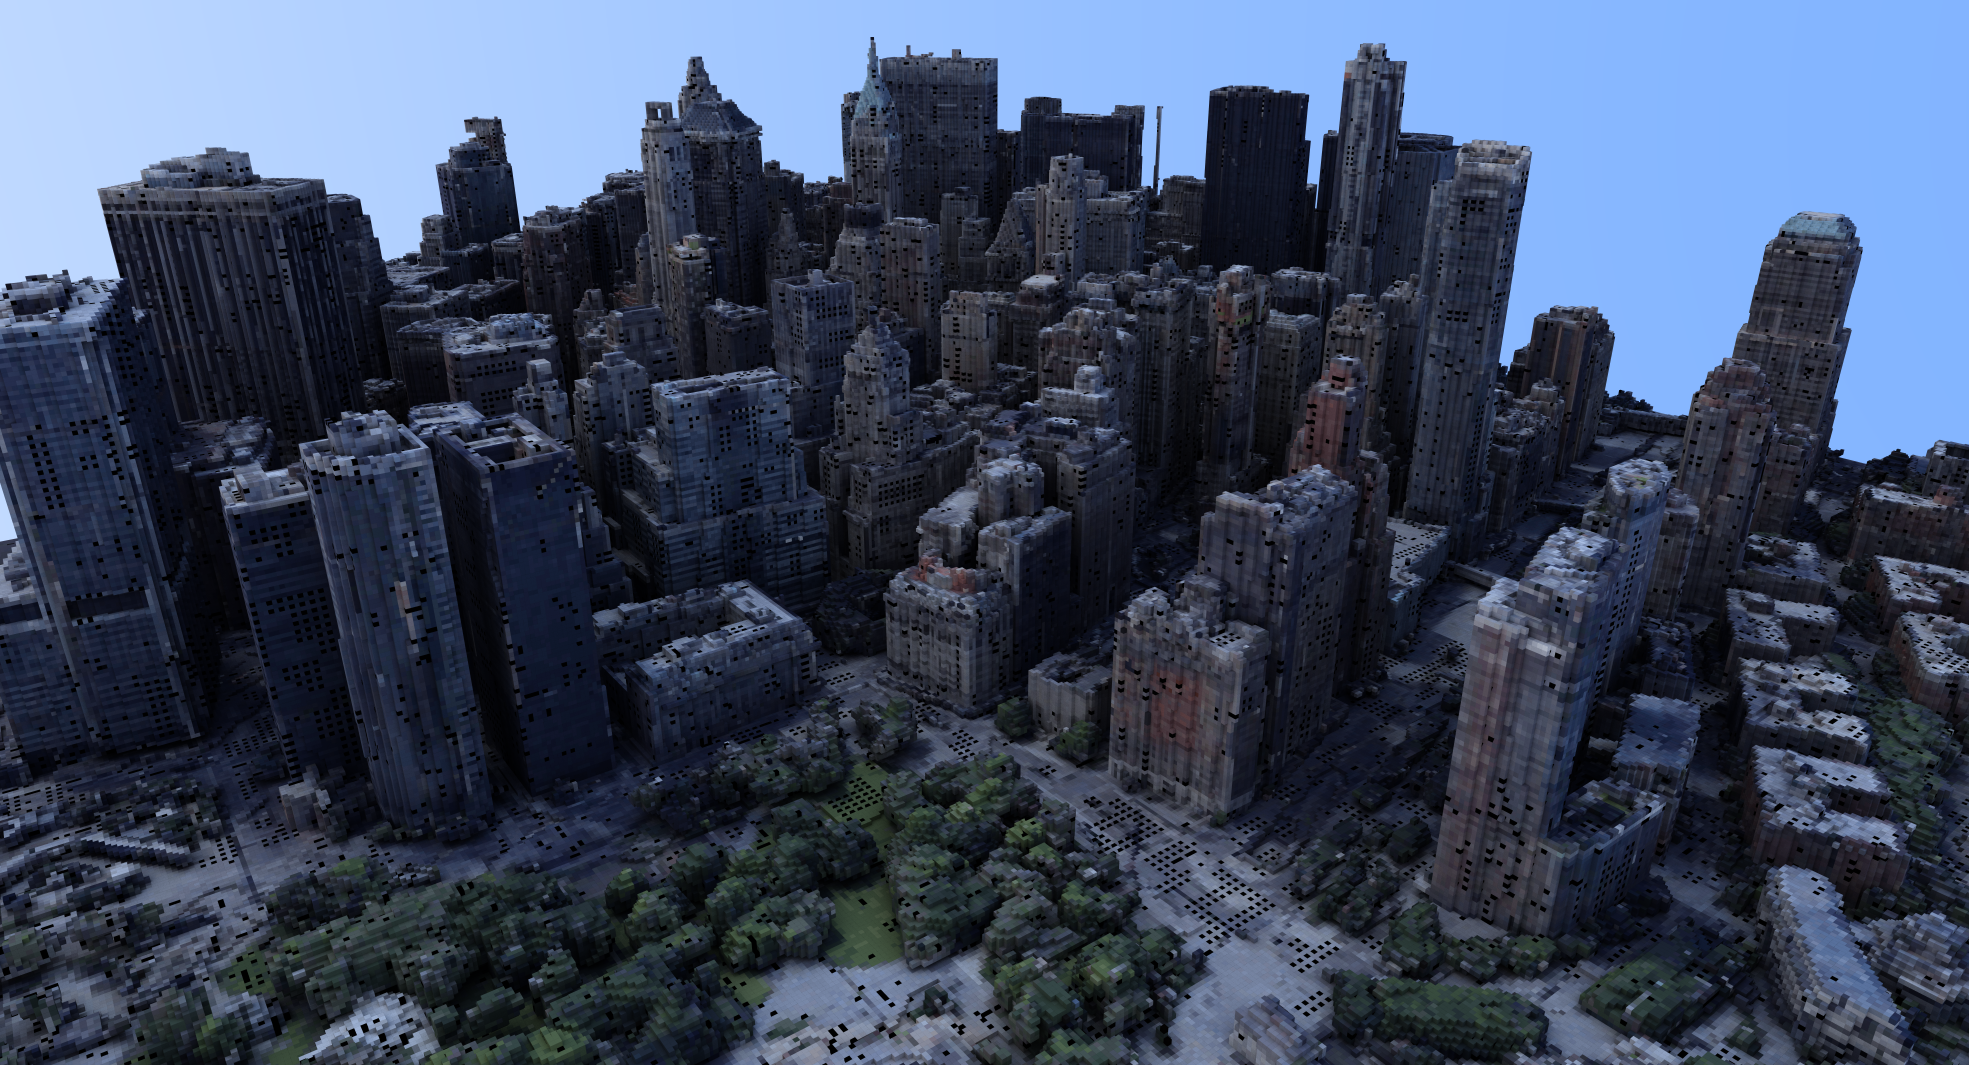
\includegraphics[scale=0.25]{NewYorkCity-Merging}
        \smallbreak
        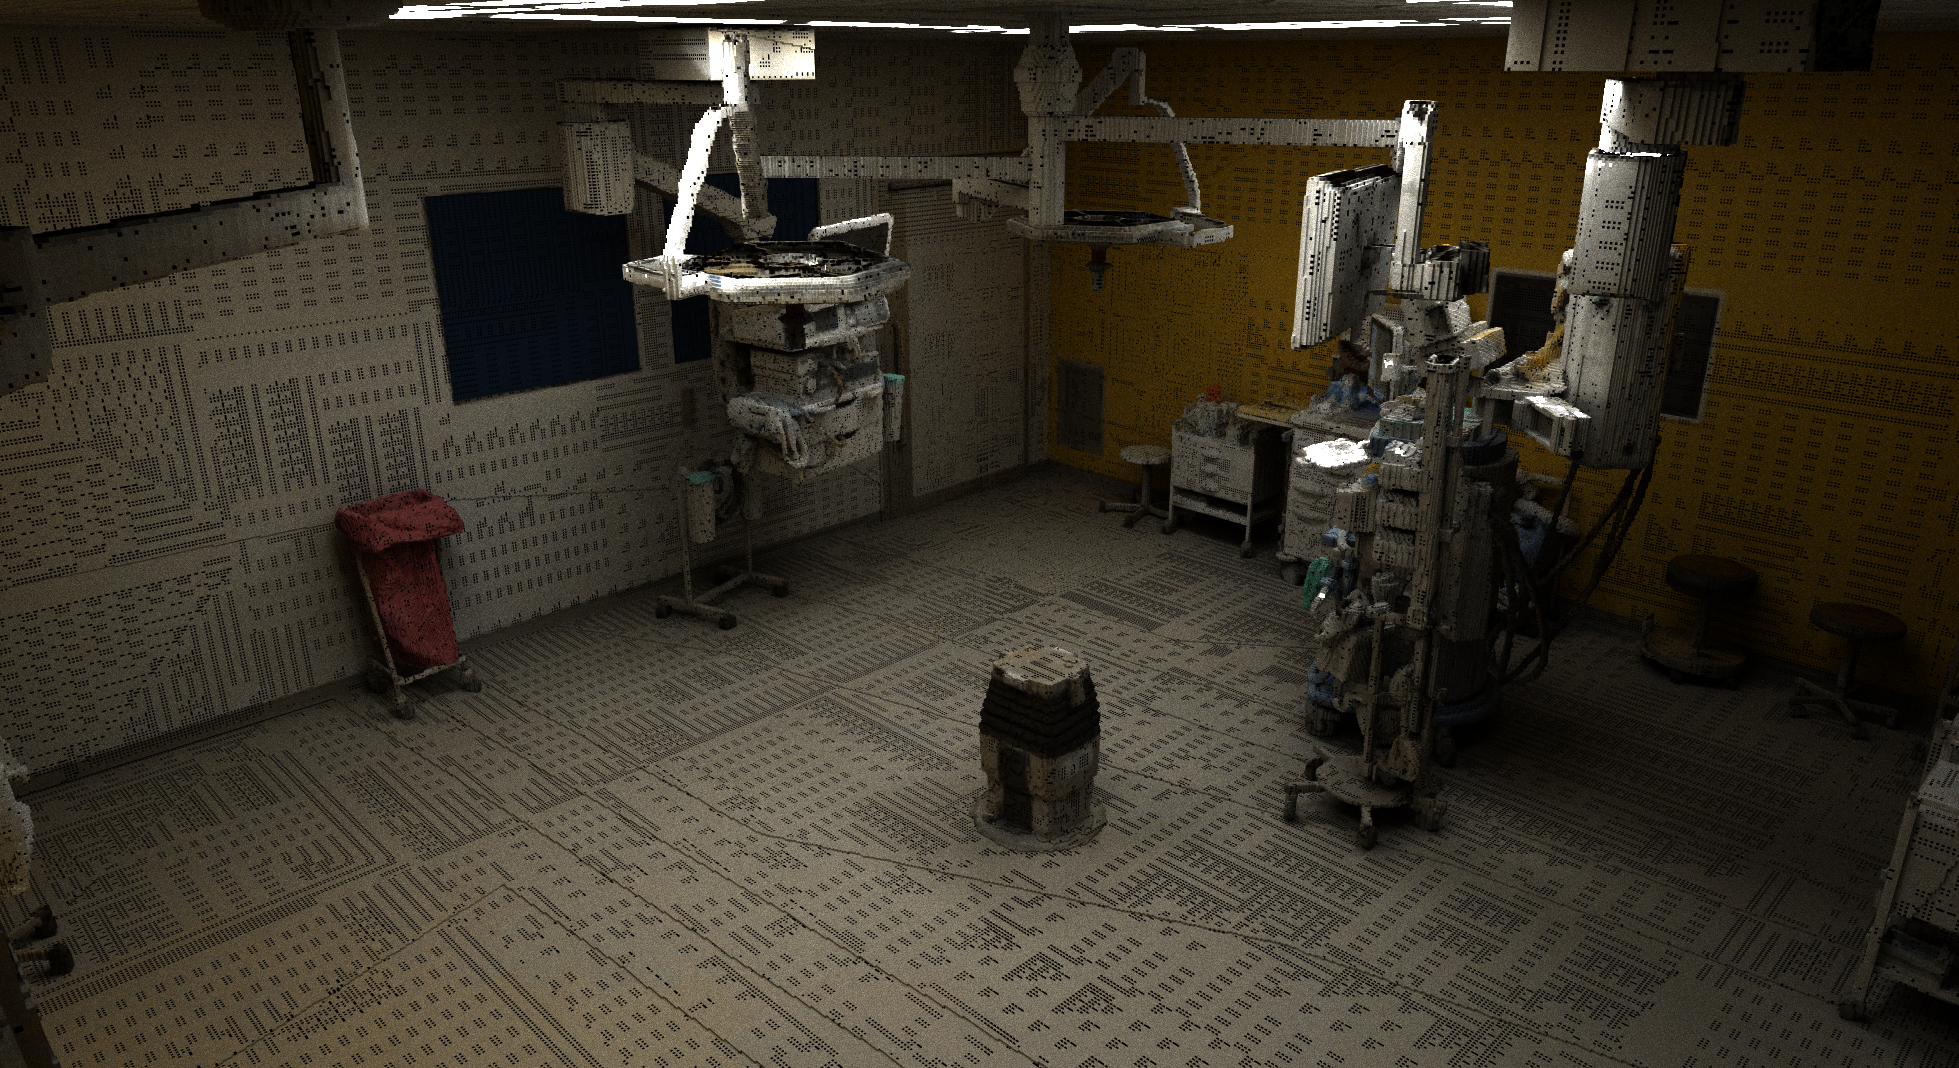
\includegraphics[scale=0.25]{OperationRoom-Merging}
    \end{center}
    \caption{
        Artifacts caused by the driver merging the AABBs.
        }
        \label{fig:Scenes-Merging}
\end{figure}

\subsection{Stability}

While collecting data, the stability of the GPU was suboptimal. The GPU crashed multiple times
during data collection and after the data was collected.
The crashes were severe, as the system had to be restarted. Most of the crashes occured
when collecting data for the Church and Operating Room. It would end prematurely before the 4096 frames were rendered.
The CPU was going through 4096 frames, however, the GPU was not presenting the frames to the screen.
The data below are from the runs that were not followed by a crash and did not cause any crashes.


\subsection{Performance Data}

\begin{table}[H]
    \centering
    \caption{Exact Intersection Performance Data}
    \vspace{0.5cm}
    \label{tab:Exact-Performance-Data}
    \begin{tabular}{c||c|c|c|}
     Scene (voxels)             & Frame Time (ms)    & Frame Per Second \\ \toprule
    New York City (4.3 mil)     & 3.07               & 324              \\
    Operating Room (5.2 mil)    & 10.7               & 93               \\
    Church (13.6 mil)           & 11.0               & 91               \\
    \end{tabular}
\end{table}

\begin{table}[H]
    \centering
    \caption{Approximate Intersection Performance Data}
    \vspace{0.5cm}
    \label{tab:Approx-Performance-Data}
    \begin{tabular}{c||c|c|c|}
     Scene (voxels)             & Frame Time (ms)    & Frame Per Second \\ \toprule
    New York City (4.3 mil)     & 3.53               & 282              \\
    Operating Room (5.2 mil)    & 10.0               & 100              \\
    Church (13.6 mil)           & 10.7               & 94               \\
    \end{tabular}
\end{table}

% Memory NYC AS:                162725888
% Memory NYC Buffer:            139198464
% Memory Operating Room AS:     195952640
% Memory Operating Room Buffer: 167706624
% Memory Church AS:             513212416
% Memory Church Buffer:         438829056

\begin{table}[H]
    \centering
    \caption{Memory Consumption in MegaBytes}
    \vspace{0.5cm}
    \label{tab:Memory-Consumption}
    \begin{tabular}{c||c|c|c|}
    Scene (voxels)              & Accel. Structure  & Voxels        & Total Memory \\ \toprule
    New York City (4.3 mil)     & 162               & 139           & 301          \\
    Operating Room (5.2 mil)    & 195               & 167           & 362          \\
    Church (13.6 mil)           & 513               & 438           & 951          \\
    \end{tabular}
\end{table}

\subsection{New York City Scene}

\begin{figure}[H]
    \begin{center}
        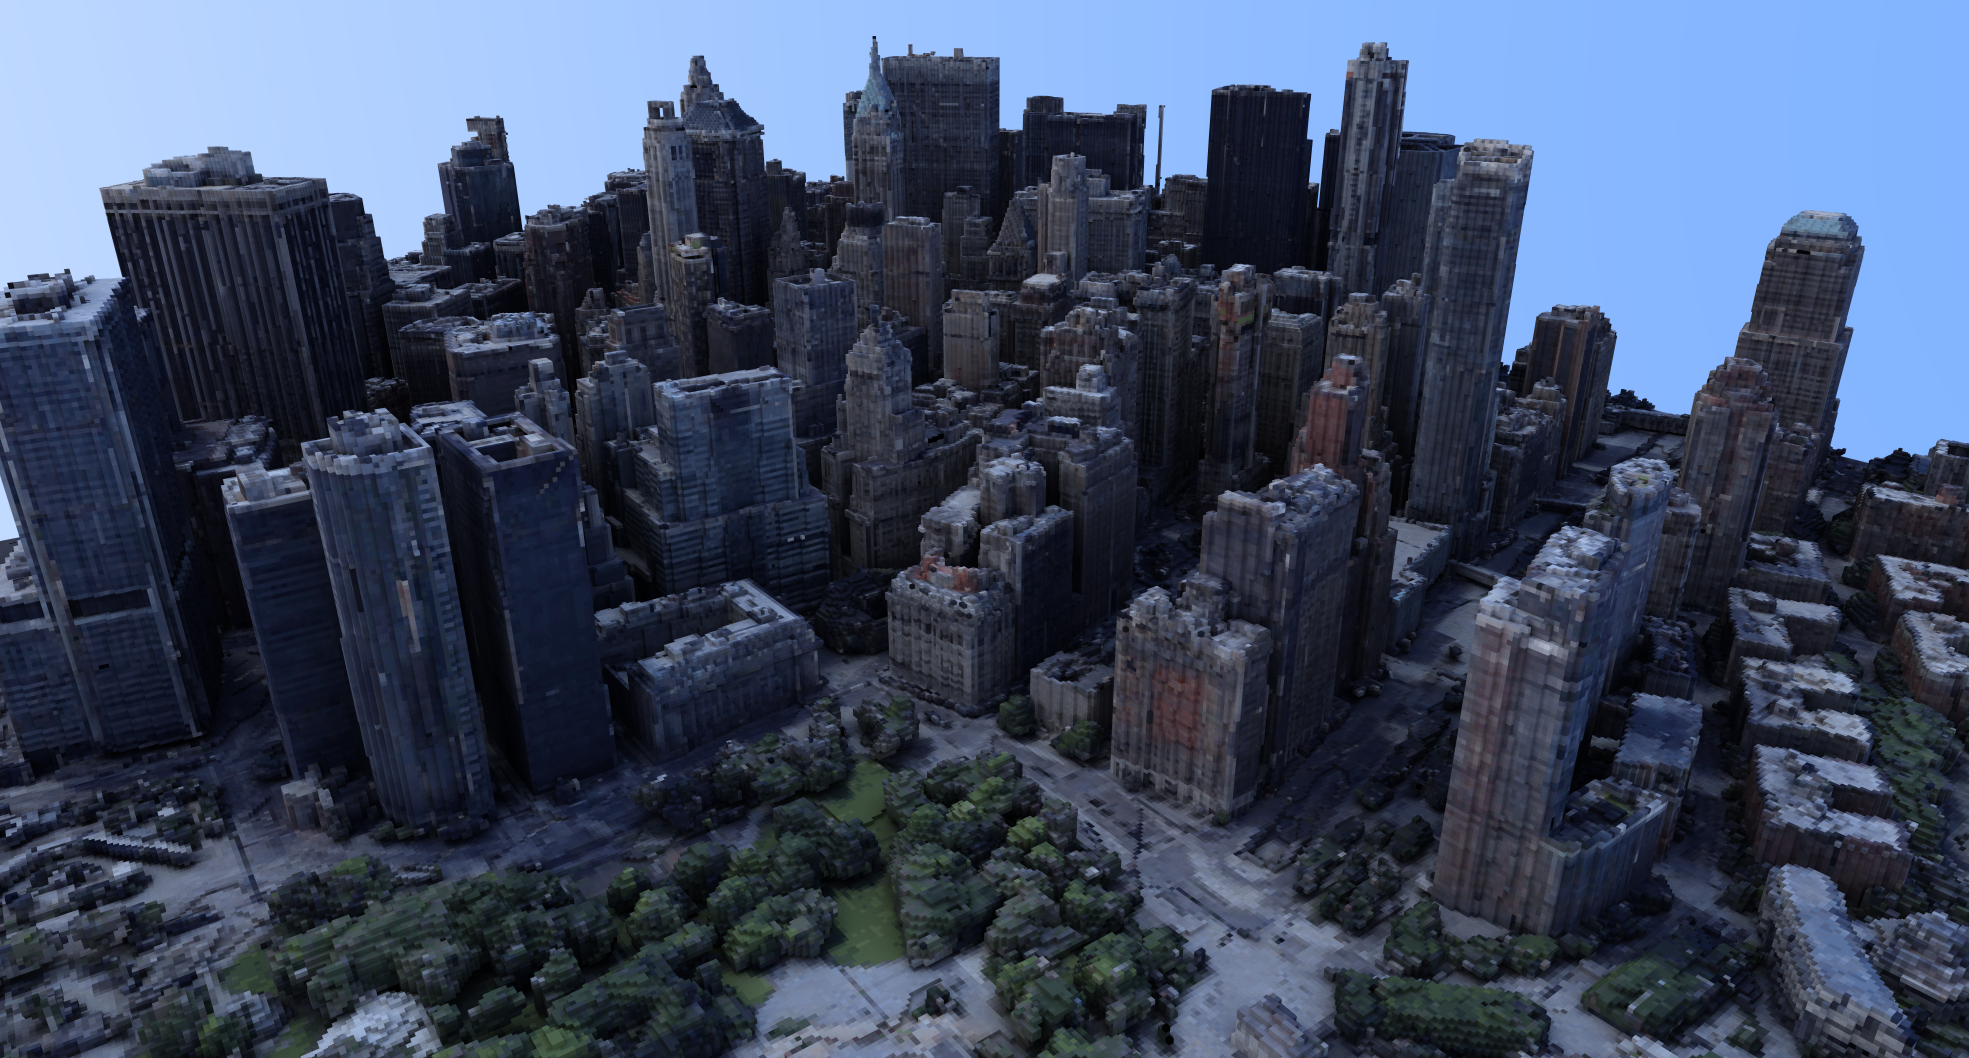
\includegraphics[scale=0.25]{NewYorkCity}
    \end{center}
    \caption{New York City Scene - Exact Intersection}
    \label{fig:NewYorkCity}
\end{figure}

Performance is optimal for the New York City scene, with 4.3 million voxels.
The exact intersection method proves to be faster than the approximate intersection method,
this is good because the exact intersection method is more accurate. Furthermore, the driver
issue discovered in the previous section does not affect the exact intersection method.
The reason behind high performance for the New York City scene is because less rays are traced.
The scene is open, meaning there it is not enclosed, hence rays can escape the scene quickly,
hitting the sky. Most of the rays do not bounce more than once or twice, which is why the performance is high.

The scene is a good representation of a real-time application, because it is open.
Most visualization application are often focusing on a single object with nothing else in the scene.
This scene could be used in a visualization application, because it is a scan of a real world location.
The frame time also gives opportunities to add more work for the GPU, such as queing Artifical Intelligence (AI) tasks,
or physics calculations. The frame time is low enough to add more work and still maintain a high frame rate.

\subsection{Operating Room Scene}

\begin{figure}[H]
    \begin{center}
        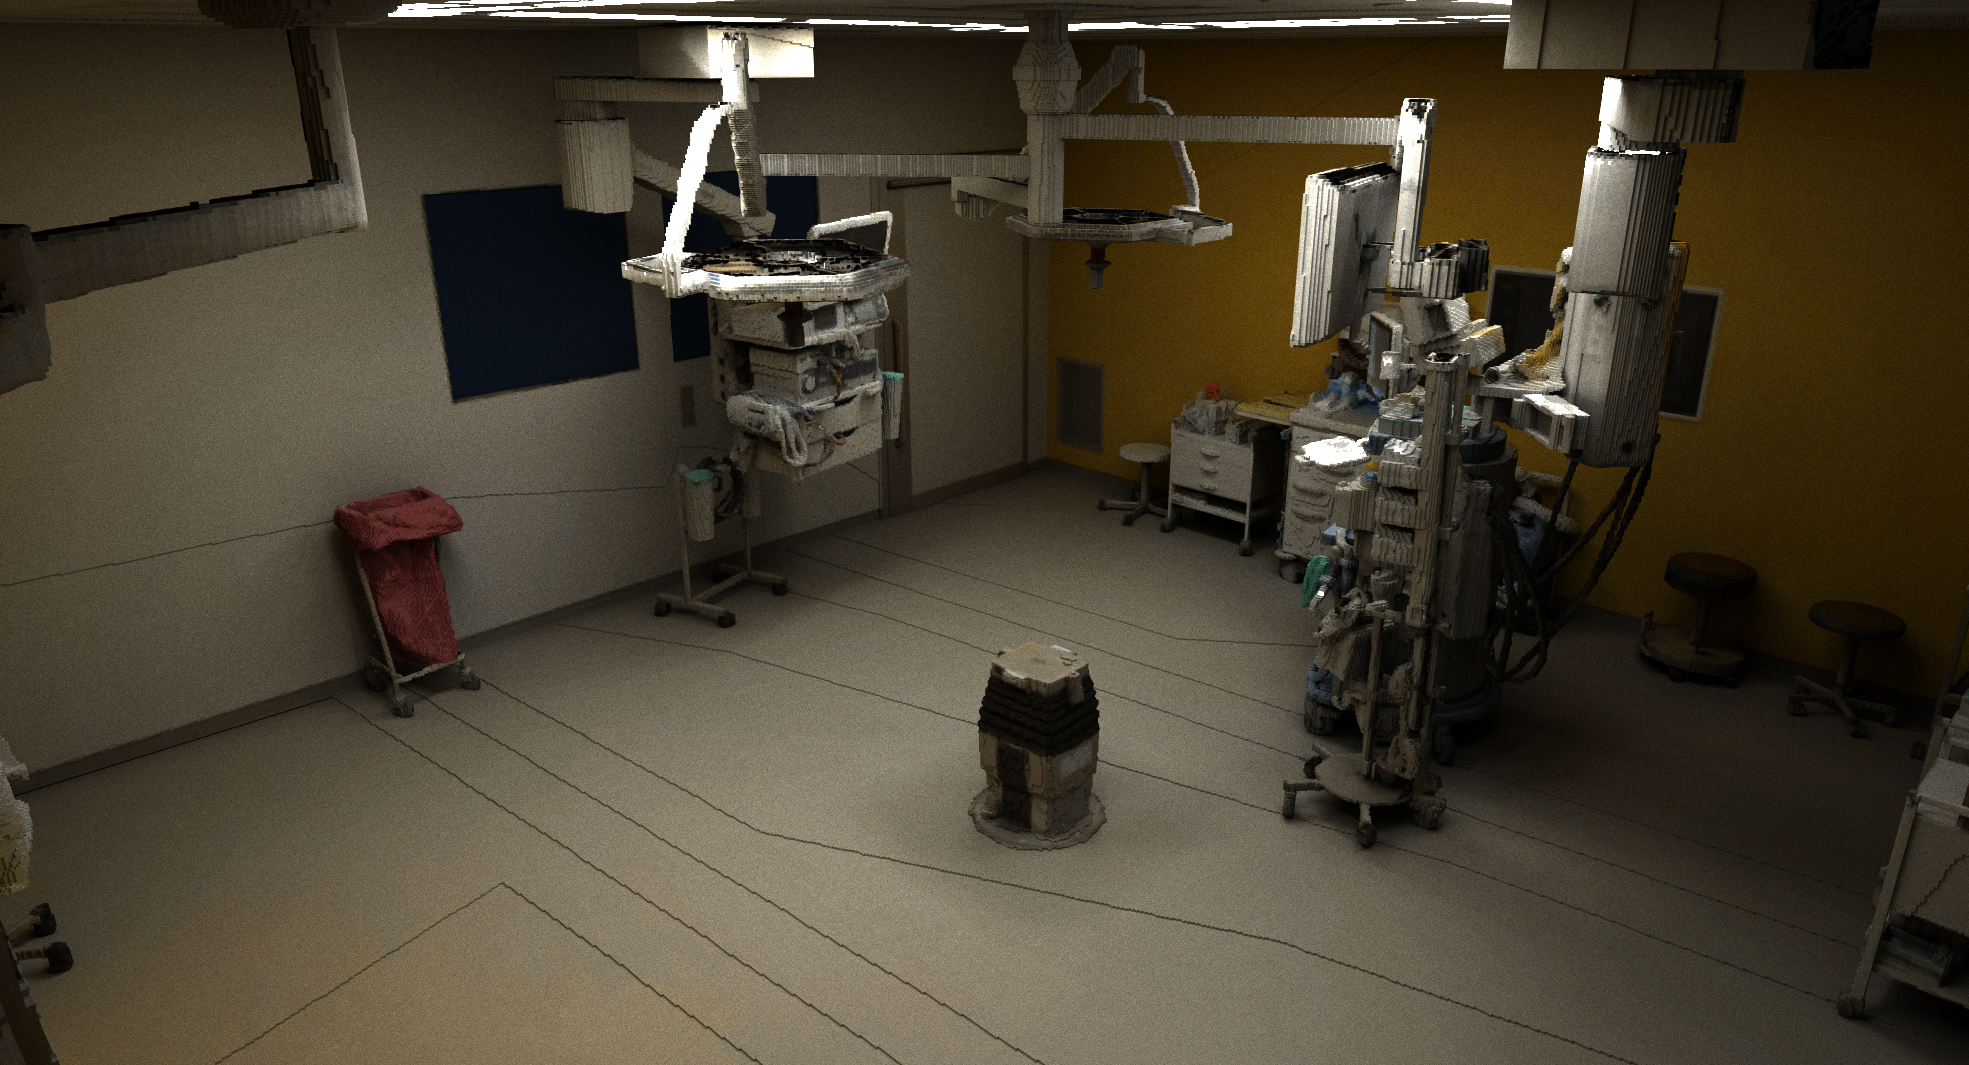
\includegraphics[scale=0.25]{OperationRoom}
    \end{center}
    \caption{Operating Room Scene - Exact Intersection}
    \label{fig:OperationRoom}
\end{figure}

Operating Room scene is a closed environment. In this scene, the frame time is considerably more than the New York City scene
which was open. This is beacuse the rays in this scene bounce more because of the closed environment
in which the rays have to bounce more to reach a light source. However, as previously mentioned 
the ray terminates itself after reaching the maximum recursion depth of 4 if it has not
hit a light source, so it is not bounding infinitely. Frame time of 10.7 for the exact intersection is reasonable and it 
leaves 6 milli seconds for extra work if the target FPS is 60. However, in this scene the optimized
intersection method is faster by 0.7 milliseconds. This scene also invokes the intersection stage
more because the rays bounce more, hence leading to more intersection tests.

Video games can have enclosed environments, and this scene is similar. The performance is optimal for this scene,
as the frames per second is above 60. Video games usually have visual effects and more work for the GPU,
which could lead to the frame rate lowering below 60. However, even considering the extra work,
the frame rate is still considered playable for a video game.

\subsection{Church Scene}

\begin{figure}[H]
    \begin{center}
        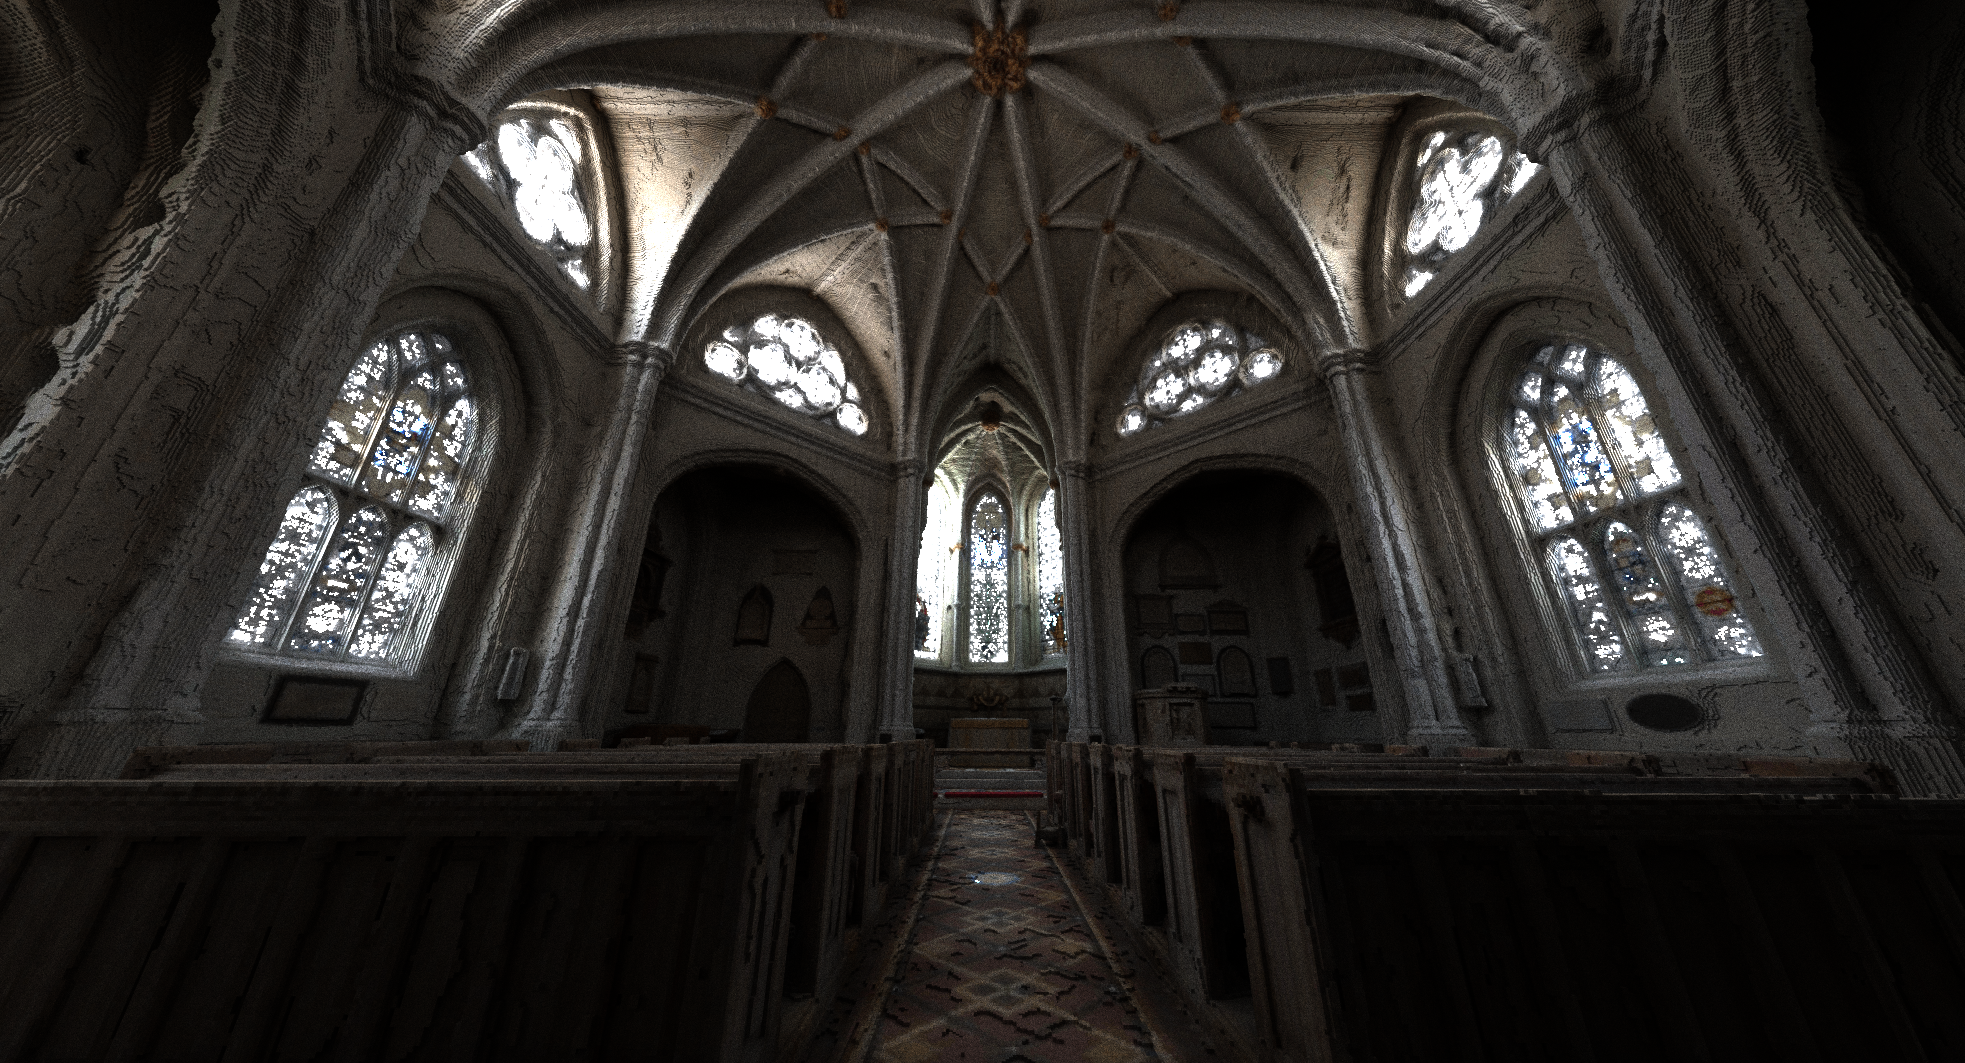
\includegraphics[scale=0.25]{Church}
    \end{center}
    \caption{Church Scene - Exact Intersection}
    \label{fig:Church}
\end{figure}

The church scene is the most complex scene with 13.6 million voxels. It is also enclosed like the operating room scene.
The frame time is 11 milliseconds, even though the scene is more complex than the operating oom scene.
Performance only differs by 0.3 milliseconds between this and the perating room scene, which is impressive.
The performance is due to the hardware accelerated BVH traversal, because it reduces the number of intersection tests logarithmically.
This means that the complexity of the scene does not linearly increase the frame time, which is excellent for real-time applications.
Optimized intersection method is also faster by 0.3 milliseconds, which is in line with the operating room scene.


Church scene is an example of an architectural visualization application, where the resolution of the geometry is high,
and the scene is enclosed.

\subsection{Memory Consumption}

The memory consumption is reasonable and low even when the scene is complex.
It is below 1GB for all the scenes, which is excellent and well within budget (4GB).
This memory consumption is also taking into account the duplicated data for the voxels. 
If there was no duplicated data, the memory consumption would have been approximately half of the total consumption in Table \ref{tab:Memory-Consumption}.


The acceleration structure has extra memory consumption, because it is a tree structure
with extra AABBs for the hierarchy. Intresting observation is that the 
acceleration structure consumes 16-17\% more memory than the raw voxel data, 
indepenedent of the scene complexity.

It is obvious that the memory consumption grows in a linear fashion with the number of voxels,
as the memory consumption is proportional to the number of voxels. 

\section{Conclusion}


The research question was: Is hardware accelerated voxel ray possible on consumer hardware for real-time applications?
Results show that hardware accelerated voxel ray is possible on consumer hardware for real-time applications.
It both handles a reasonable number of voxels that would be used in real-time applications and does not exceed the memory budget.
The performance also leaves room for other tasks such as AI, physics calculations and post processing which are common in real-time applications.
Increase in scene complexity does not scale linearly with the frame time, which allows for even more complex scenes
to be ray traced than the ones used in this essay. Maybe even upwards of 100 million voxels in real time. 

The optimization method in this essay does improve frame time in closed environments but not in open environments.
However, the optimization method is not practical on NVIDIA GPUs because the driver does not conform to the specification.
The difference 0.3-0.7 milliseconds is not significant. The optimization is worth only if the driver issue is resolved,
because it is simpler.

\printbibliography

\end{document}